\usetikzlibrary{decorations.markings}
\newif\iflabrev

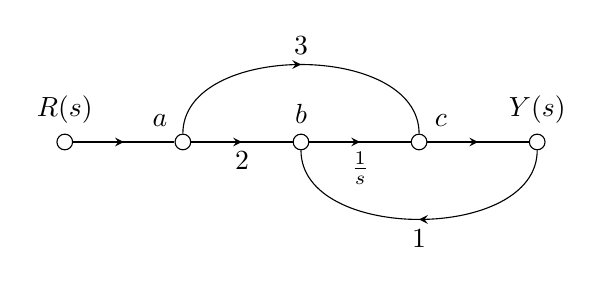
\begin{tikzpicture}
[
label revd/.is if=labrev,
%label revd/.default=true,
amark/.style={
            decoration={             
                        markings,   
                        mark=at position {0.5} with { 
                                    \arrow{stealth},
                                    \iflabrev \node[above] {#1};\else \node[below] {#1};\fi
                        }
            },
            postaction={decorate}
},
terminal/.style 2 args={draw,circle,inner sep=2pt,label={#1:#2}},
]

%Place the nodes
\node[terminal={above}{$R(s)$}] (a) at (0,0) {};
\node[terminal={above left}{$a$}] (b) at (1.5,0) {};
\node[terminal={above}{$b$}] (c) at (3,0) {};
\node[terminal={above right}{$c$}] (d) at (4.5,0) {};
\node[terminal={above}{$Y(s)$}] (e) at (6,0) {};
%Draw the connections
\draw[amark](a) to (b);
\draw[amark=$2$] (b) to (c);
\draw[amark=$\frac{1}{s}$] (c) to (d);
\draw[amark=$3$,label revd] (b) to[bend left=90] (d);
\draw[amark] (d) to (e);
\draw[amark=$1$] (e) to[bend left=90] (c);
\end{tikzpicture}
